\section{Theorie}
\label{sec:Theorie}


\subsection{Grundlagen}
Ultraschalltechnik ist heutzutage sehr präsent in der Medizin und Werkstoffprüfung.
Schallwellen im Frequenzbereich von etwa $\SI{20}{\kilo\hertz}$ bis $\SI{1}{\giga\hertz}$, welche oberhalb der menschlichen Hörschwelle liegen, werden Ultraschall genannt.
In Gasen und Flüssigkeiten äußern sie sich wegen Druckschwankungen in Longitudinalwellen der Form
\begin{equation}
  p(x,t) = p_0 + \nu_0 Z cos{\omega t -kx},
\end{equation}
wobei $Z = c \cdot \rho$ die akustische Impedanz des Mediums beschreibt, welche von der Schallgeschwindigkeit (Phasengeschwindigkeit) $c$ und der Dichte $\rho$ des Mediums abhängt.
Die Phasengeschwindigkeit $c$ hängt jedoch in Flüssigkeiten von ihrer Kompressibilität $\kappa$ und Dichte $\rho$ ab, für sie gilt
\begin{equation}
  c_{\text{Fl}} = \sqrt{\frac{1}{\kappa \cdot \rho}}.
\end{equation}
In Festkörpern bilden sich zusätzlich aufgrund von Schubspannungen Transversalwellen aus.
Hier ist die Phasengeschwindigkeit
\begin{equation}
  c_{\text{Fe}} = \sqrt{\frac{E}{\rho}}
\end{equation}
abhängig von dem Elastizitätsmodul des Festkörpers.
In der Regel sind die Phasengeschwindigkeiten der Transversal- und Longitudinalwellen unterschiedlich.\\
Für die Ultraschalltechnik sind zwei Aspekte relevant.
Zunächst, dass die Schallintensität beim Durchlaufen eines Mediums durch Absorption exponentiell abnimmt.
Für die Intensität ergibt sich
\begin{equation}
  I(x) = I_0 \cdot \exp(\alpha x). \label{gl:1}
\end{equation}
Da der Absorptionskoeffizient $\alpha$ beispielsweise in Luft sehr klein ist, wird in der Medizin oftmals ein Kontaktmittel zwischen Probe und Schallsender eingesetzt.\\
Der zweite Aspekt ist, dass Schallwellen die gleichen physikalischen Eigenschaften haben wie elektromagnetische Wellen, wie zum Beispiel die Reflexion an Grenzflächen.
Wenn eine Ultraschallwelle auf eine Grenzfläche stößt, wird ein Teil reflektiert.
Das Verhältnis zwischen reflektierter und einfallender Intensität beschreibt der Reflexionskoeffizient
\begin{equation}
  R = \left(\frac{Z_1-Z_2}{Z_1+Z_2}\right)^2,
\end{equation}
welcher aus den akustischen Impedanzen der beiden Grenzflächen bestimmt wird.
Für den Transmissionskoeffizienten gilt $T = 1 - R$.

\subsection{Erzeugung von Ultraschallwellen}
Ultraschall kann beispielsweise mit Hilfe des piezo-elektrischen Effekts erzeugt werden.
Hierzu wird ein piezoelektrischer Kristall, zum Beispiel Quarz, in einem elektrischen Wechselfeld zu Schwingungen angeregt.
Dabei emittiert dieser Ultraschallwellen.
Umgekehrt kann der Kristall auch als Empfänger dienen, indem er von Ultraschallwellen angeregt wird.

\subsection{Anwendungsverfahren}
Es wird generell zwischen zwei Methoden unterschieden, dem Durchschallungs-Verfahren und dem Echo-Impuls-Verfahren.
Beide basieren auf einer Laufzeitmessung, bei der ein Schallimpuls ausgesendet wird, welcher auf einer definierten Messstrecke nach zu messender Zeit am Empfänger ankommt.\\
Beim Durchschallungsverfahren, Abbildung \ref{abb:1}, wird an einer Seite der Probe ein Schallimpuls eingesendet, welcher am anderen Ende der Probe durch einen Empfänger aufgenommen wird.
Befindet sich nun eine Fehlstelle in der Probe, wird ein signifikanter Intensitätsverlust beobachtet.
Aussagen über die Position der Fehlstelle können nicht getroffen werden.\\
Beim Echo-Impuls-Verfahren, dargestellt in Abbildung \ref{abb:2}, dient der Sender gleichzeitig als Empfänger.
An Grenzflächen wird die Ultraschallwelle reflektiert und wird dann registriert.
Bei einer Fehlstelle wird letztendlich ein vorzeitiges Intensitätsmaximum aufgenommen, welches Aufschluss über die ungefähre Größe und Tiefenposition jener gibt.
Für die Tiefe $s$ gilt der Zusammenhang
\begin{equation}
  s = \frac{ct}{2},
\end{equation}
sie ist demnach von der Laufzeit $t$ und der Phasengeschwindigkeit $c$ abhängig.

\begin{figure}[H]
  \centering
  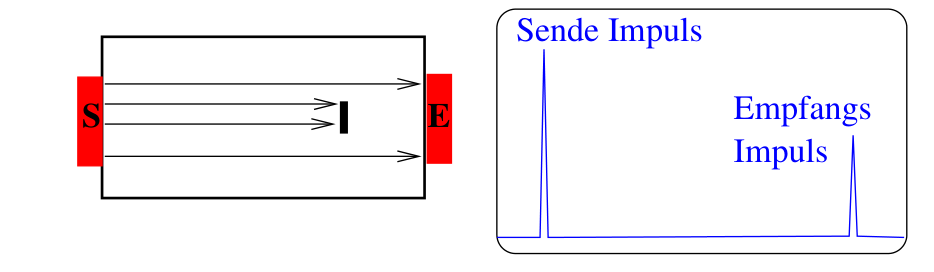
\includegraphics[height=4cm]{ressources/durch.png}
  \caption{Darstellung des Durchschallungsverfahrens. \cite{skript}}
  \label{abb:1}
\end{figure}

\begin{figure}[H]
  \centering
  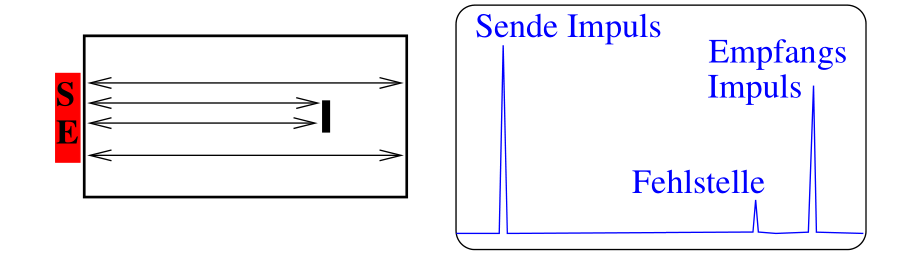
\includegraphics[height=4cm]{ressources/echo.png}
  \caption{Darstellung des Echo-Impuls-Verfahrens. \cite{skript}}
  \label{abb:2}
\end{figure}



% 2x2 Plot
% \begin{figure*}
%     \centering
%     \begin{subfigure}[b]{0.475\textwidth}
%         \centering
%         \includegraphics[width=\textwidth]{Abbildungen/Schaltung1.pdf}
%         \caption[]%
%         {{\small Schaltung 1.}}
%         \label{fig:Schaltung1}
%     \end{subfigure}
%     \hfill
%     \begin{subfigure}[b]{0.475\textwidth}
%         \centering
%         \includegraphics[width=\textwidth]{Abbildungen/Schaltung2.pdf}
%         \caption[]%
%         {{\small Schaltung 2.}}
%         \label{fig:Schaltung2}
%     \end{subfigure}
%     \vskip\baselineskip
%     \begin{subfigure}[b]{0.475\textwidth}
%         \centering
%         \includegraphics[width=\textwidth]{Abbildungen/Schaltung4.pdf}    % Zahlen vertauscht ... -.-
%         \caption[]%
%         {{\small Schaltung 3.}}
%         \label{fig:Schaltung3}
%     \end{subfigure}
%     \quad
%     \begin{subfigure}[b]{0.475\textwidth}
%         \centering
%         \includegraphics[width=\textwidth]{Abbildungen/Schaltung3.pdf}
%         \caption[]%
%         {{\small Schaltung 4.}}
%         \label{fig:Schaltung4}
%     \end{subfigure}
%     \caption[]
%     {Ersatzschaltbilder der verschiedenen Teilaufgaben.}
%     \label{fig:Schaltungen}
% \end{figure*}
